\section{Software Technology Stack}
\label{sec:technology}

This section of the report will cover each of the chosen software technologies that are implemented in the final project application. It will introduce some of key concepts of the technologies, with some running examples. 

\subsection{Firebase}
\label{sub:firebase}
Firebase is a Backend-as-Service (BaaS) platform created by Google that provides helpful tools. Examples of these are:

\begin{itemize}
 \item \textbf{Firebase Database:} Is a NoSQL cloud database used for storing and syncing data. The data is synced in realtime and remains available even when the application goes offline. The data is stored as JSON. \cite{firebasedb}
 \item \textbf{Firebase Cloud Firestore:} Cloud database with good scalability for mobile, web and server development. Cloud Firestore offers flexibility, expressive querying, realtime updates and more. \cite{firebasefs}
 \item \textbf{Firebase Cloud Messaging:} Used to send notification/data messages. \cite{firebasecm}
 \item \textbf{Firebase Remote Config:} Used to quickly update/change behavior and appearance of your application without having to download an update. \cite{firebaserc}
\end{itemize}
As for the poll application that was made in the project it only uses the Cloud Firestore out of these four. In the Cloud database the data is stored in documents with underlying collections where all values are stored in a structural way. In Figure~\ref{fig:fb} the data is stored in such a way, with IDs as the document name and the values are stored in collections with fields for each value. The database supports many different data types, from integers and strings to more complex data in the form of objects.
\begin{figure}[H]
  \centering
  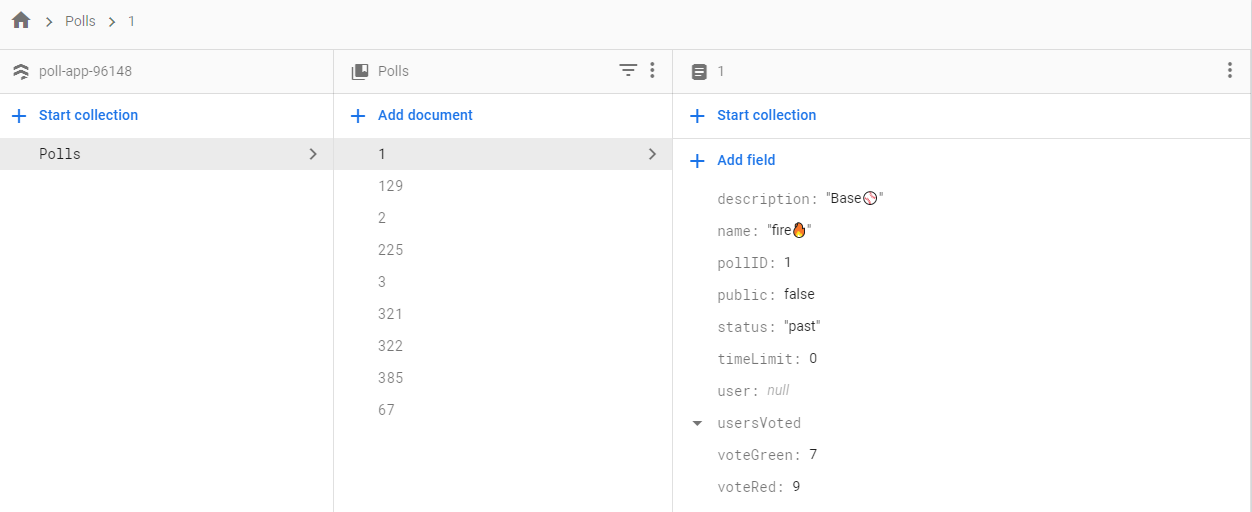
\includegraphics[scale=0.4]{figs/fb.png}
  \caption[scale=0.5]{Firebase Cloud Firestore.}
  \label{fig:fb}
\end{figure}

\subsection{RabbitMQ}
\label{sub:rabbitmq}

RabbitMQ is an open source message broker that implements Advanced Message Queuing Protocol (AMQP). RabbitMQ is an intermediary for messaging. “It gives your applications a common platform to send and receive messages, and your messages a safe place to live until received.” \cite{rabbitftrs}
How this works is that a producer publishes messages to the “exchange” with specific type of exchange, the exchange then delivers the messages to different queues depending on exchange types. The recipients will then retrieve messages which they have subscribed to.

\subsection{Spring framework}
\label{sub:spring}
\subsubsection{Thymeleaf}
Thymeleaf is a template engine written in Java for HTML5/XHTML/XML. It can be used in both web and non-web environments. Thymeleaf implements the concept of Natural Templates, that are described as: “template files that can be directly opened in browsers and that still display correctly as web pages” \cite{thymlf}. The use of Thymeleaf can act as a replacement for using Java Server Pages \cite{javaserverpages}.
\subsubsection{Spring Boot}
Spring Boot allows for creating Spring based applications in an “easy” way that just runs, with minimal effort. Spring Boot does a lot of the configuration for the user by being a framework built on top of Spring framework which enables the user to quickly “bootstrap” a Spring application from scratch. The Spring initializer makes for an effortless start to any project by simply picking out dependencies according to the type of project.
\subsubsection{Spring JPA}
Spring JPA is a framework provided by Spring, to make it easier for developers to implement data access layer. By letting the developer only have to write the entities, repository interfaces, and perhaps making some extra custom repository searching methods. While the developer is focusing on programming the vision of the project, Spring JPA will implement all necessary methods for accessing all the data from repositories for the developer.
\subsubsection{Spring MVC}
Spring MVC is the framework used to build the web application. It provides the Model-View-Controller architecture. This simply means that it separates the application into a model, view, and controller component. The task of these components is to handle different sides of the development in an application. When it comes to creating scalable projects, Model-View-Controller is one of the most commonly used web development frameworks.
\subsubsection{Spring Security}
Spring Security is a powerful and highly customizable authentication and access-control framework. It is the the most used and a practical standard for securing Spring-based applications, thus also our application. Spring Security is a framework that focuses on providing both authentication and authorization to Java applications.\cite{springsecurity} Security is very important and should not be taken for granted. In this aspect, Sprint Security makes it very easy to customize and tweak the settings to meet the developers preferences. Features available to customize is a long list, but protection against attacks and authentication with access-control (AC), are the few features that are featured in our FeedApp application.
\subsection{Dweet.io}
\label{sub:dweet}
Dweet.io is a type of messaging system for machines. It is also referred to as a “Twitter for social machines” \cite{dweet}. A machine can either publish or subscribe to data, and all data published to dweet.io can be retrieved by simply calling an URL. All messages published to dweet.io will be associated with an unique name. The data is structured in JSON format. 

\subsection{H2 Database}
\label{sub:h2db}
H2 Database is an open-source SQL database written in Java. The database can be embedded in Java applications, making it a suitable choice for development and testing. The database engine is also exceptionally fast. \cite{h2db} 

The H2 console allows for a full view of the database. It allows for SQL commands for inspecting/or changing values in the database, as is seen in figure~\ref{fig:h2console}. After starting an application with H2 embedded in it, the console can be reached in a browser by calling the path URL that is configured. If the application is running on port 8080, and the path URL is set to /h2-console, simply call “localhost:8080/h2-console”. After inputting the correct username and password, one is free to inspect and manage values the database. 
\begin{figure}[H]
  \centering
  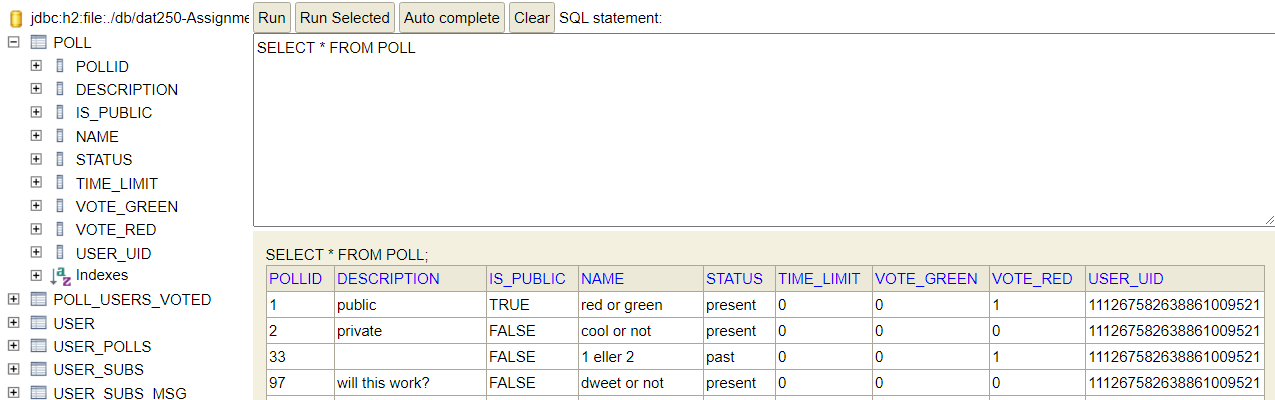
\includegraphics[scale=0.45]{figs/h2cons.png}
  \caption[scale=0.5]{A SQL command is run in the H2 console.}
  \label{fig:h2console}
\end{figure}